\documentclass[conference,10pt]{IEEEtran}
\IEEEoverridecommandlockouts
\usepackage[T1]{fontenc}
\usepackage{graphicx,booktabs,amsmath,amssymb,xcolor,url,xspace}
\usepackage[hidelinks]{hyperref}
\hypersetup{pdftitle={Egocentric Human Demonstrations for a Bimanual Robot: Methods and Pipeline}, pdfauthor={Jeong Hwan Lee}}
\usepackage{tikz}
\usetikzlibrary{positioning,arrows.meta}
\newcommand{\mm}{\,mm\xspace}
\def\UrlBreaks{\do\/\do\_\do\.\do\-}\def\UrlFont{\small\ttfamily}\newcommand{\code}[1]{\path{#1}}

\begin{document}
\title{Egocentric Human Demonstrations for a Bimanual Robot\\Methods and Pipeline}
\author{\IEEEauthorblockN{Jeong Hwan Lee}
\IEEEauthorblockA{Technical report, version 4, 7 October 2026 \quad alnrg2arg@gmail.com\\
Companion to Part I (three-cube stacking) and Part II (single-arm approach). Describes how each stage works, not its results.}}
\maketitle

\begin{abstract}
This document describes, at the level of algorithms, parameters and gates, every stage we used to turn egocentric human
demonstrations into robot policies: the hand-worn recording rig and collection protocols, sensor and robot calibration,
synchronisation and export, monocular wrist-pose recovery and the three metric-scale sources (IMU, a cube of known size and a
table plane), two generations of conversion into robot training data (joint-space retargeting and a Cartesian action contract),
the single-arm variant with a shared task frame, the X-VLA model and its training recipes, the offline and diagnostic
evaluations, and deployment on the robot. File names refer to the repository unless stated otherwise. The last section lists
inconsistencies we found in our own code while writing it.
\end{abstract}

\section{Overview}
Fig.~\ref{fig:overview} shows the stages. Each stage writes its output with a manifest and is followed by a gate that either
accepts a unit (episode, segment, row or take) or rejects it with a reason; the reports count what each gate removes. Two
conversions share the front end: generation~1 (Gen-1) retargets human wrist poses to robot joint trajectories, and generation~2
(Gen-2) expresses them in the same relative Cartesian action space as our robot teleoperation data. The single-arm approach data
(Part II) is a Gen-2 variant with masked dimensions and a physical origin shared with the robot.

\begin{figure*}[t]
\centering
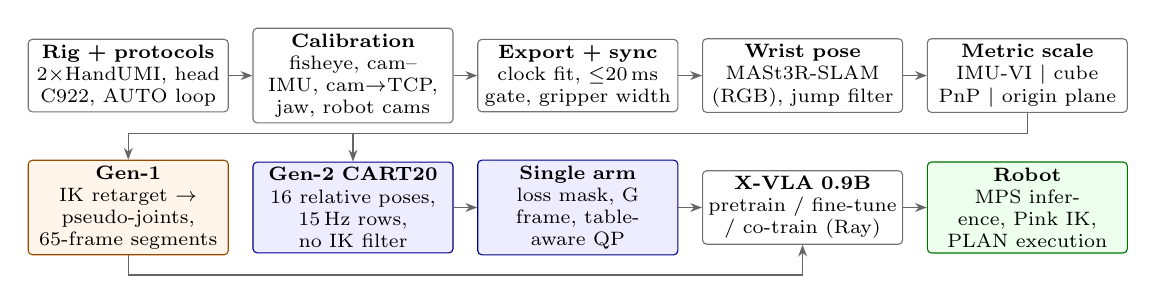
\begin{tikzpicture}[font=\scriptsize, node distance=3mm and 3mm,
  box/.style={draw=black!55, rounded corners=1.5pt, align=center, inner sep=2pt, minimum height=9mm, text width=24mm, fill=white},
  g1/.style={box, fill=orange!8, draw=orange!60!black}, g2/.style={box, fill=blue!7, draw=blue!55!black},
  dep/.style={box, fill=green!7, draw=green!45!black}, arr/.style={-{Stealth[length=1.5mm]}, draw=black!60}]
\node[box] (rig) {\textbf{Rig + protocols}\\2$\times$HandUMI, head C922, AUTO loop};
\node[box, right=of rig] (cal) {\textbf{Calibration}\\fisheye, cam--IMU, cam$\to$TCP, jaw, robot cams};
\node[box, right=of cal] (exp) {\textbf{Export + sync}\\clock fit, $\le$20\,ms gate, gripper width};
\node[box, right=of exp] (pose) {\textbf{Wrist pose}\\MASt3R-SLAM (RGB), jump filter};
\node[box, right=of pose] (scale) {\textbf{Metric scale}\\IMU-VI $\mid$ cube PnP $\mid$ origin plane};
\node[g1, below=6mm of rig] (g1) {\textbf{Gen-1}\\IK retarget $\to$ pseudo-joints, 65-frame segments};
\node[g2, right=of g1] (g2) {\textbf{Gen-2 CART20}\\16 relative poses, 15\,Hz rows, no IK filter};
\node[g2, right=of g2] (hra) {\textbf{Single arm}\\loss mask, G frame, table-aware QP};
\node[box, right=of hra] (train) {\textbf{X-VLA 0.9B}\\pretrain / fine-tune / co-train (Ray)};
\node[dep, right=of train] (dep) {\textbf{Robot}\\MPS inference, Pink IK, PLAN execution};
\draw[arr] (rig)--(cal); \draw[arr] (cal)--(exp); \draw[arr] (exp)--(pose); \draw[arr] (pose)--(scale);
\draw[arr] (scale.south) |- ++(0,-2.6mm) -| (g1.north); \draw[arr] (scale.south) |- ++(0,-2.6mm) -| (g2.north);
\draw[arr] (g2)--(hra); \draw[arr] (hra)--(train); \draw[arr] (train)--(dep);
\draw[arr] (g1.south) |- ++(0,-2.5mm) -| (train.south);
\end{tikzpicture}
\caption{Pipeline overview. Orange: generation 1 (joint space); blue: generation 2 (Cartesian) and its single-arm variant; green:
deployment. Every arrow is followed by a gate with a logged reason.}
\label{fig:overview}
\end{figure*}

\section{Recording Rig and Collection Protocols}\label{sec:rig}
\textbf{Rig} (\code{collection/configs/handumi/hardware_handumi_v1.yaml}). Each HandUMI unit carries an Arducam fisheye UVC
camera (1920$\times$1080, 30\,fps, MJPG), an ICM-42688-P IMU on a Teensy~4.1 (nominal 200\,Hz; measured 201.6 and 197.9\,Hz
because each board has its own oscillator) and a Feetech STS3215 servo used as a jaw encoder (4096 ticks/rev, polled at
100\,Hz). Both wrist cameras report the same USB serial, so they are matched by product name. A fixed Logitech C922
(640$\times$480, 30\,fps, autofocus off) records the table; an RGB-D camera was dropped because it disrupted the wrist streams.

\textbf{Recording} (\code{collector/recorder.py}). An episode directory holds one MP4 per camera, \code{sensors.mcap},
\code{events.json} and \code{episode_meta.json}; it is renamed from \code{.incomplete} to \code{.complete} only when closed.
MCAP JSON channels carry IMU samples (device and host timestamps, accelerometer, gyro), gripper samples (unwrapped and wrapped
ticks, normalized value), per-frame metadata (frame index, capture time, skipped frames), events and clock anchors. All streams
are stamped with the host monotonic clock: the IMU at host receive time, the gripper at the midpoint of the serial
transaction, frames at capture.

\textbf{AUTO loop} (\code{collector/autoloop.py}). A state machine RESET $\to$ ARMING $\to$ HOLD $\to$ (PREP) $\to$ EPISODE
$\to$ STOP drives each take with spoken cues. ARMING waits for stillness: in 0.25\,s windows the mean gyro magnitude must be
below 6\textdegree/s, the accelerometer-magnitude standard deviation below 0.35\,m/s$^2$, the largest sample gap below 25\,ms and
the window at least 60\% filled, for a continuous run of 1\,s. A hold after recording starts gives the visual--inertial
initialisation window. A take that passes preliminary QA is kept automatically; a failure pauses the loop.
\begin{itemize}
\item \emph{Stacking}: 20\,s takes, 10\,s reset, 3\,s hold; the next order is the one with the fewest kept takes
(\code{episode_manager.next_order}), so orders are balanced rather than randomized.
\item \emph{Robot-like} (\code{robot_like_v1}): 30\,s takes with live feedback. Wrist angular speed and angular acceleration
on a 15\,Hz grid are compared with the 95th percentiles of robot teleoperation data (0.996\,rad/s, 4.413\,rad/s$^2$); a take is
sent to review if more than 10\% of ticks exceed them or fewer than two grasps occur.
\item \emph{Approach} (HRA\_red): right hand only, 10\,s takes, 5\,s reset, gripper checks off.
\item \emph{Approach with origin} (HRA\_A100): 5\,s rest; 2\,s still with the jaw tip on a taped cross; recording starts with a
further 2\,s origin hold (event \code{go_cue}); a 3\,s ``ready'' move to a robot-like start; at ``go'' a 10\,s approach. The
right wrist also records a robot-camera-like view.
\end{itemize}

\textbf{Collection QA} (\code{collector/integrity.py}). A take goes to review on device or recorder error events, an empty
stream, or a frame rate below 25\,fps; it is rejected if the gripper is sampled below 20\,Hz, frozen, outside its calibrated
span by more than 300 ticks, or travels less than 5\% of its range. Validation decodes every video to its metadata frame count
and checks that frame indices are contiguous and capture times strictly increasing.

\section{Calibration}\label{sec:cal}
\textbf{Wrist cameras.} Kannala--Brandt (equidistant) fisheye models at full resolution, fitted with Kalibr on an 8$\times$5
checkerboard of 25\mm squares (left $f_x{=}788.9$\,px). \textbf{Camera--IMU.} Kalibr~\cite{furgale2013kalibr} extrinsics and time
offsets per hand. \textbf{Camera to TCP} (\code{calibration/camera_tcp/handumi_camera_tcp_v2.yaml}). The TCP is the pinch
centre with $x$ along the approach direction, $y$ along jaw closing and $z = x\times y$. The rotation is a fixed axis permutation
($x_\text{TCP}=z_\text{cam}$, $y_\text{TCP}=-x_\text{cam}$, $z_\text{TCP}=-y_\text{cam}$); the translation comes from caliper
measurements (95\mm forward, 95\mm down) rotated by the camera pitch measured from IMU gravity (20.7\textdegree), giving
$t=(0, 55.3, 122.5)$\mm, consistent to about 1\mm with a cube-based fit. It was measured on one unit and applied to both.
\textbf{Head camera.} A provisional plumb-bob model ($f=677.7$\,px).

\textbf{Robot side} (Part II). The robot's fixed camera is calibrated on the same checkerboard ($f=728.7$\,px, RMS 1.05\,px); the
right jaw tip touches four inner corners, the forward-kinematics (FK) TCP positions and the board pose from PnP give
$T_\text{base,board}$ by Kabsch alignment, and $T_\text{base,cam}=T_\text{base,board}T_\text{cam,board}^{-1}$. The robot
wrist camera is calibrated from 13 board views (intrinsics with fixed aspect, no tangential distortion, RMS 0.16\,px) and its
hand-eye transform is solved with the Tsai, Park, Horaud and Daniilidis methods~\cite{tsai1989handeye}; Park's solution is used.
Physical contact is modelled by the URDF fingertip box (70--80\mm behind the IK TCP along $x$, $\pm$19.6\mm in $z$), whose
lowest corner counts as the contact point.

\section{Export and Synchronisation}\label{sec:export}
\textbf{Clock alignment} (\code{pose/timing.py}). IMU device time is mapped to host time by a least-squares slope with the
intercept re-anchored at the 5th percentile of the residuals, because USB latency only ever adds delay; the camera--IMU time
offset from calibration is then applied. Cameras free-run at slightly different rates (30.003--30.026\,Hz), so frames are paired
by nearest capture time rather than by a constant offset.

\textbf{Export} (\code{pipeline/export/umi_export_orbslam.py}). Each wrist is written as a 960$\times$540 video (intrinsics
halved), an IMU file in GoPro-telemetry layout with 50\,ms of IMU before the first frame, and a camera settings file; frames and
capture times come from a single decoding pass so they cannot drift apart.

\textbf{Synchronisation gate} (\code{pipeline/census/c8_census_pre.py}, \code{c8_phase3.py}). The left wrist is the master
clock; the right wrist and the head camera are matched by nearest capture time. A row is valid if both wrist poses are valid and
both matches are within 20\,ms ($\Delta t_R<20$\,ms and $\Delta t_H<20$\,ms). An episode passes if it contains at
least one run of 65 consecutive valid rows.

\textbf{Gripper width} (\code{pipeline/grip/}). Each frame takes the nearest gripper sample. Because the recorded normalized value
was unreliable (the open end lay beyond the mechanical stop and the left direction flipped between sessions), Gen-1 recomputes
the width from raw ticks: direction from the open/closed tick pair, a closed anchor from per-episode closed extremes, the open end
at the closed anchor plus the device span (1136.6 / 1248.2 ticks), and width $= \mathrm{clip}(f,0,1)\times 67.5$\mm. Gen-2 uses a
later caliper calibration (gcal1): piecewise-linear knots at 0/20/40/60/80\mm, normalized as $g=\mathrm{clip}(w/80\,\text{mm},0,1)$,
0 = closed.

\section{Wrist Pose and Metric Scale}\label{sec:pose}
\textbf{Monocular pose} (\code{pipeline/mast3r_pose/run_perframe.py}). MASt3R-SLAM~\cite{murai2025mast3rslam} (official
code, pinned commit; the only patch is a build fix) runs on the RGB wrist video undistorted to a pinhole view, single-threaded,
every frame, fixed seed. After global optimisation every frame is re-expressed on its final keyframe:
\begin{equation}
T_{WC}(f) = T_{WK}^{\text{final}}(k)\,T_{WK}^{\text{track}}(k)^{-1}\,T_{WC}^{\text{track}}(f),
\end{equation}
a Sim(3) chain; frames tracked during relocalisation are invalid unless they later became keyframes. The UMI approach of one
ORB-SLAM3 map per scene~\cite{chi2024umi} was replaced because it failed to relocalise after scene changes.

\textbf{IMU visual--inertial scale} (\code{cp6_scale.py:imu_vi}). The SLAM trajectory is metric up to a per-episode scale $s$.
With $R_{wb}=R_{wc}R_{cb}$, accelerometer samples $f_b$ box-averaged around each frame, the camera acceleration $a_\text{cam}$ and
the lever-arm acceleration $a_\text{lever}$ obtained as Savitzky--Golay second derivatives (order 3, window $W$) of the SLAM camera
position and of $R_{wc}t_{cb}$, each frame contributes three rows of
\begin{equation}
R_{wb}\,f_b - a_\text{lever} = s\,a_\text{cam} - g\;\;(+\,R_{wb}b_a),
\end{equation}
solved for $s$ and $g\in\mathbb{R}^3$ by Huber-weighted iteratively reweighted least squares (10 iterations, $\sigma=1.4826\,$MAD)
over the longest valid run. Both sides pass the same filter, so they share the band limit, and nothing is integrated twice.
$W=15$ without bias was selected on a fit split of the marker benchmark. A scale is valid if $s>0$, $|g|\in[8.81,10.81]$\,m/s$^2$
and $s$ lies within 0.1$\times$ the smallest and 10$\times$ the largest benchmark scale. Metric TCP poses are $T_\text{tcp}=
(T_{WC}\text{ with translation}\times s)\,X_\text{cam,tcp}$.

\textbf{Pose benchmark.} 14 demonstrations (28 hand tracks; 9 for fitting, 5 held out) with four 80\mm ArUco markers in view.
Marker poses are solved with IPPE on undistorted points; markers more than 20\textdegree{} from the consensus are rejected.
Ground-truth scale is the median ratio of marker to SLAM displacement over frame pairs ten frames apart in which a marker moved
more than 30\mm. Reported: coverage, scale error, rotation error, a UMI-style 16-step relative position error and the rate of
direction reversals.

\textbf{Camera--IMU consistency.} Sessions whose gyro and SLAM angular velocities disagree (median cosine near 0 against
0.92--0.98 elsewhere) are quarantined. For the approach data, the exported camera--IMU rotation of the right wrist was corrected by
about 18\textdegree{} about the camera $x$ axis after comparison with the cube and table geometry.

\textbf{Pose-jump filter} (\code{cart20/ego_cart20/preprocessing/pose_filter.py}). MASt3R-SLAM occasionally moves the camera by
centimetres within one frame without a loss flag. A raw step is flagged when the displacement over one 66.7\,ms row exceeds 100\mm{}
or 45\textdegree{} and the jump lies in that step, or when a step above 50\mm is isolated between steps slower than 0.3\,m/s.
Flags within 5 samples form one event. If the pose returns (within $\max(30\,\text{mm}, 0.3\times\text{step})$ and 45\textdegree)
the event is a spike and only its samples are invalidated; otherwise it is one-way and the rest of that arm's track is
invalidated, because a start-anchored state would be wrong from then on.

\textbf{Cube PnP scale} (\code{cart20/ego_cart20/cube_pnp.py}; Part II). For slow motions the IMU fit is unobservable. The red
cube (edge 38\mm) is segmented in HSV, its convex hull reduced to six (or four) vertices whose corners are sharpened by line fits
to the middle of each side, and fitted by PnP with two- and three-face silhouette models (with a visibility check: the faces the
camera lies in front of must equal the model's visible faces) or, within 35\textdegree{} of head-on, a single-face IPPE model with
the centre placed half an edge behind the face. Since the cube is static, its centre $c_i=p_i + k\,R_i t_i$ must be constant, which
gives the inverse scale in closed form,
\begin{equation}
k = -\frac{\sum_i (p_i-\bar p)\cdot(u_i-\bar u)}{\sum_i\lVert u_i-\bar u\rVert^2},\qquad u_i=R_i t_i,\quad s=1/k,
\end{equation}
with MAD trimming and 200 bootstrap resamples. A take needs at least 10 PnP frames, a bootstrap spread of at most 10\% and a
centre residual of at most 2\,cm.

\textbf{Origin-plane scale} (Part II, HRA\_A100). During the origin hold the fingertip touches the plate, so the first SLAM keyframe
sees the table at a known distance. Excluding the finger region and low-confidence points, up to three planes are fitted by RANSAC
(400 iterations, threshold 0.4\% of the median depth) and the largest one parallel to the first is taken as the table; then
$s=|n\cdot t_\text{tip}|/(s_0\,|d|)$ with $t_\text{tip}$ the fingertip in camera coordinates and $s_0$ the keyframe's Sim(3) scale.
Cube PnP is used when valid, otherwise the plane.

\section{Generation 1: Joint-Space Retargeting}\label{sec:gen1}
\textbf{Segments and gates} (\code{c8_phase3.py}). Valid rows are cut into non-overlapping 65-frame blocks (2.17\,s). Per arm, a
segment must have a valid metric scale (B), keep at least 95\% of rows inside the robot workspace (C; a target is inside if its
nearest neighbour among 6{,}000 robot teleoperation TCP poses is within 50\mm{} and the smallest of the 50 nearest orientation
differences is below 20\textdegree), solve IK on every row (D) and yield finite joints (E). A segment is bimanual if both arms
pass.

\textbf{Retargeting} (\code{pipeline/pseudo_joint/pseudo_joint_pipeline.py}). Human motion is taken relative to the segment start
and mapped into the robot dataset's TCP frame, $\text{rel}=F^{-1}T_{0}^{-1}T_{t}F$ with $F=R_x(180^\circ)$, and placed at a fixed
robot anchor posture (the median active posture of robot teleoperation data): $T_\text{tgt}=\mathrm{FK}(q_\text{anchor})\,C^{-1}\,
\text{rel}\,C$, $C=R_y(90^\circ)$. A least-squares IK (pose cost with orientation weight 20, a rest term towards the previous
solution, joint-limit constraints, at most 10 iterations, joint step at most 0.35\,rad) is seeded from the previous row; rows are
labelled LIMIT, DQ\_FAIL ($>$1\,rad), BRANCH\_SWITCH ($>$0.3\,rad while the target barely moves), NOT\_CONVERGED ($>$15\mm{} or
$>$5\textdegree) or OK.

\textbf{Dataset and targets} (\code{pipeline/dataset/}, \code{training/humanik_delta.py}). One LeRobot episode per segment: three
640$\times$480 views, a 14-D state (six joint angles and a gripper value per arm) and the target TCP poses. The policy predicts 30
cumulative joint displacements $a_i=q_{t+5+i}-q_t$ (a 5-frame lead) and an absolute binary gripper. Two auxiliary losses tie joint
space to the measured motion: (C) the relative TCP translation $\mathrm{trans}(T_\text{tgt}(t)^{-1}T_\text{tgt}(t{+}5{+}i))\times10$
in spare action dimensions, and (D) an FK consistency term,
\begin{equation}
\mathcal{L}=\mathcal{L}_{\Delta q}+\mathcal{L}_\text{grip}+2.0\,\mathcal{L}_C+20\,\lVert \mathrm{FK}(q_t+\hat a)-p_\text{tgt}\rVert^2 .
\end{equation}
The split draws 10\% of source episodes with a fixed seed; no episode spans both sides.

\textbf{Retargeting v2} (\code{pipeline/retarget_v2/}). The single anchor made every segment start from one posture. v2 uses only
30 robot episodes for calibration (evaluating on 120 others). A seed bank of $2^{17}$ Sobol samples of both arms' joints is filtered
by workspace, table floor, manipulability (smallest singular value of the position Jacobian) and inter-arm clearance $\ge$75\mm{}
(exact segment-to-segment distances between 9 link segments per arm), then de-duplicated (1{,}195 seeds). Variant K rolls out the
best 8 seeds and scores $S=\overline{e_\text{pos}}/15+\overline{e_\text{rot}}/5+\overline{|\Delta q|}/0.6+0.5\,\overline{|\Delta^2q|}/0.6$;
Kr adds the posture distance to robot data; TR retrieves the 64 nearest robot trajectory windows by a 96-D relative-motion
feature, keeps feasible ones and seeds IK with $q_\text{last}+\Delta q_\text{ref}$. A hybrid keeps TR when feasible, otherwise Kr.

\section{Generation 2: The Cartesian Contract (CART20)}\label{sec:gen2}
\textbf{Contract} (\code{cart20/ego_cart20/config.py}). Rows at 15\,Hz; offsets $\Delta=3/59.94$\,s $=50.05$\,ms, the robot data's
step. For row time $t$ and each arm,
\begin{equation}
A_k = T(t)^{-1}\,T(t+k\Delta),\qquad k=1,\dots,16 ,
\end{equation}
current-anchored (not sequential), interpolated on the raw 30\,Hz track (linear position, SLERP rotation, linear gripper; only
between valid samples at most 50\,ms apart; no extrapolation). Each arm contributes [position 3 $\mid$ 6-D rotation (the first two
rows of $R$, decoded by Gram--Schmidt) $\mid$ gripper], so two arms give 20 dimensions; the model's 32-D action is padded with 12
dimensions that are exactly zero. The state is each arm's pose relative to its own task-start pose, $T(t_0)^{-1}T(t)$, plus both
grippers (there is no shared left--right SLAM frame).

\textbf{Conversion} (\code{convert.py}). Pose-jump filter; per-arm interpolation tracks; task start at the first instant both arms
are valid; nearest head frame within 20\,ms. A row is a training row only if both arms are valid at $t$, all 16 targets are valid
and a head frame exists; there is no padding. No workspace or IK selection is applied.

\textbf{Validation} (\code{validation/}, \code{tests/}). Shapes, zero padding, finite values, $g\in[0,1]$, orthonormal rotations with
determinant $+1$, identity start state, disjoint splits, no target beyond the last valid row, and median translation increasing with
$k$; eleven synthetic tests pin the contract.

\textbf{Robot-like wrist rendering} (\code{scripts/export_lerobot_robotized.py}). To narrow the visual gap, a fisheye frame is
re-rendered as a virtual pinhole camera with the same orientation (so labels stay valid): horizontal field of view drawn from
62--70\textdegree, principal point shifted 75--125\,px down so the jaws sit low as on the robot, then downscaled, blurred
($\sigma$ 0.4--1.0), JPEG-compressed (quality 55--85) and photometrically jittered, with a per-frame seed. ROBOT100 applies it to
every frame. The single-arm robotcam v2 rendering (Sec.~\ref{sec:hra}) instead uses the measured robot camera.

\textbf{Export.} LeRobot v3 at 15\,fps, three 224$\times$224 views, statistics recomputed (padding dimensions mean 0, std 1); the
joint fields are NaN on purpose so that any joint-space loss fails loudly.

\section{Single-Arm Variant and Shared Task Frame}\label{sec:hra}
\textbf{Right-only contract} (\code{right_only.py}). The tensor layout is unchanged: the left state is the identity pose with
gripper 0, the left action is zero motion, and a per-episode 20-D loss mask supervises only the right arm's position and rotation
(9 dimensions; the gripper was static and masked).

\textbf{Robot-camera rendering} (robotcam v2). For each robot-camera pixel, the ray from the measured robot intrinsics is projected
into the fisheye model and resampled (rays outside the fisheye view are black), with small focal and principal-point jitter and the
same degradation chain. Labels are moved from the UMI TCP to the robot TCP through the hand-eye transform, $T_\text{robot}=T_\text{UMI}M^{-1}$.

\textbf{Task frame G.} Three robot jaw-tip touches on the taped line give the origin (cross centre), $x$ along the tape and $z$ along
base $z$. At the human side, the origin pose is the median position and mean rotation over the hold; its yaw is measured per take by
matching table features around the cross (ORB, ratio test, PnP-RANSAC) against a reference take, with tilt from IMU gravity
(corrected extrinsic). The state is then the absolute pose in G and labels are $T_G = T_{\text{base},G}\,R(\text{yaw})\,
T_\text{origin}^{-1}T_\text{robot}$.

\textbf{Table-aware conversion.} The human trajectory is warped from its own start towards a chosen robot start pose $T_S$ with
smoothstep weights $\mathrm{sst}(x)=3x^2-2x^3$ over normalized time $s$: $w_{xy}=1-\mathrm{sst}((s-0.2)/0.6)$, $w_z=1-\mathrm{sst}(s/0.3)$,
$w_\text{rot}=1-\mathrm{sst}((s-0.1)/0.5)$, so the endpoint near the cube is the human's. A height correction $c$ is then solved
per take as a quadratic program,
\begin{equation}
\begin{aligned}
\min_c\;& \textstyle\sum c^2+50(\Delta c)^2+2000(\Delta^2 c)^2+60\,m\,(c-g)^2\\
\text{s.t.}\;& z_\text{tip}+c\ge z_\text{table}+5\,\text{mm},
\end{aligned}
\end{equation}
with $c_0=0$, the endpoint lift at most 30\mm{} and $g$ pulling low frames towards 12\mm{} clearance. The result is replayed through
IK (every second frame; error below 5\mm{} and 3\textdegree, joint margin above 2\textdegree). Takes are classed PASS (lift
$\le$20\mm), PASS-CORRECTED (20--30\mm), REVIEW, EXCLUDED or REJECT (IK success below 98\%, missing origin hold or yaw, hold moved
more than 10\mm, start below the floor); only the first two are exported.

\section{Model}\label{sec:model}
X-VLA~\cite{zheng2025xvla} through LeRobot~\cite{cadene2024lerobot}: a Florence-2~\cite{xiao2024florence2} vision-language encoder,
a 24-layer soft-prompted transformer (hidden 1024, 16 heads) and a flow-matching~\cite{lipman2023flow} action head; about 0.9B
parameters, all trainable. Inputs are three views resized with padding to 224$\times$224, the instruction (BART tokenizer) and the
proprioceptive state. \textbf{Soft prompts.} An embedding table of 30 domains $\times$ 32 tokens is appended to the sequence, and the
state/action projections are domain-specific linear layers; the domain id is set in the checkpoint's preprocessor. Reading the
public weights showed that only domains 10--17 had ever been trained; we use the unused domain 20 for our embodiment.
\textbf{Flow matching.} Training draws stratified $t$, forms $x_t=\varepsilon t+a(1-t)$ and regresses the clean action $a$
directly. Inference starts from $x_1\sim\mathcal N(0,I)$ and for $i=N\dots1$ sets $t=i/N$, $x_t=x_1 t+\hat a(1-t)$, $\hat a=f(x_t)$,
reusing $x_1$ (10 steps by default). \textbf{Widening for Gen-2.} The public head (20-D action and state) was widened to a 32-D
action and 20-D state: existing rows are copied exactly, new rows drawn from the base rows' scale, new biases zero, and the widened
model checked to reproduce the base for every domain.

\section{Training}\label{sec:train}
\textbf{Gen-1} (\code{training/train_bi.py}). The joint-displacement target and losses of Sec.~\ref{sec:gen1}, AdamW (learning
rate $10^{-4}$, the vision-language group at 0.1$\times$, weight decay $10^{-4}$, gradient clip 10), 1k warm-up and cosine decay to
$2.5\times10^{-6}$, batch 4, fp32 with TF32, 300k steps, a checkpoint every 10k. A 20-step smoke run must log finite losses and
active auxiliary terms first. The checkpoint selection rule (minimum geo score on validation) was fixed before training.

\textbf{Gen-2, REL-only} (\code{training/relonly/}). The loss is the MSE on action dimensions 0--19; the transformer is patched so that
dimensions 20--31 are zero at its input and output at every denoising step, in training and at inference. A preflight checks that the
loss ignores randomized padding targets, that padding predictions are exactly zero and that their decoder gradients vanish. 8-bit
AdamW (bitsandbytes) with a save shim, bf16 autocast with fp32 master weights, batch 8, seed 1000, warm-up 1k, cosine decay ending
exactly at the last step (the launcher refuses runs whose step count and decay differ, because LeRobot silently rescales the
schedule). Actions are mean/std-normalized, states not. \textbf{Loss mask} (single arm): masked targets are replaced by the detached
prediction before subtraction (avoiding NaN gradients) and the loss is normalized by the number of supervised elements.
\textbf{Fine-tuning} starts a fresh optimizer from the pretrained weights and uses the robot dataset's normalization statistics;
episode subsets (e.g.\ R30) are selected by index list. \textbf{Co-training} draws exactly four ego and four robot samples per batch.

\textbf{Operations.} Jobs are submitted to a Ray cluster and pinned to a GPU node (RTX~4090 or RTX~5090; their PyTorch versions
differ, so cross-node runs are not bit-identical). Launchers refuse to start on a busy GPU, a code-hash or domain-id mismatch, a
failed gripper-contract gate or low disk space, and a disk guard stops training before the node fills. A 60-step smoke run (with
save and resume) precedes each main run. An archiver copies every checkpoint to external storage with SHA-256 verification before
deleting it from the node, keeping optimizer state only at fixed intervals.

\section{Evaluation}\label{sec:eval}
\textbf{Gen-1 offline} (\code{evaluation/c8old_mac_eval.py}). On held-out episodes, seven start frames per segment (every 5 frames
in 0--30); one flow sample per start with a fixed seed. For horizons $k\in\{1,4,8,16,30\}$: TCP error $\lVert\mathrm{FK}(q_t+\hat
a_k)-p_k\rVert$ (median, p90), joint MAE, the MAE of a zero-motion predictor, and the cosine of predicted versus measured TCP
displacement. The geo score is the mean of median TCP errors over horizons; a collapse ratio compares prediction and target spread.
The moving subset requires at least 20\mm{} of TCP motion by $k{=}30$. \textbf{Prompt swap}: each sample is run with all six order
instructions under one seed and with the true instruction under two more seeds; instruction spread is compared with seed spread,
and the true instruction's error rank among the six with chance. \textbf{Paired bootstrap}: episode-level resampling (10k draws,
identical for both models) of the relative difference in geo score between two initializations.

\textbf{Gen-2 diagnostics} (\code{analysis/v3/}). Teacher-forced direction cosine on robot frames (predicted versus recorded
translation at $k$=4/8/16 for frames moving more than 10\mm), repeated under all left/right swaps and axis sign flips; an image/state
domain swap (ego or robot images combined with ego, robot or zero state); optical-flow versus pose-axis correlation of the wrist
videos (a convention check); and wrist-image sharpness as the variance of the Laplacian. \textbf{Training-loss comparisons}: losses
are parsed from logs (step = line index $\times$ log interval) and compared as window means and ratios. \textbf{Held-out loss}
(single arm): the training loss (masked) on all validation rows with two noise seeds and on a 2{,}000-row training subset.

\textbf{Claim verification} (\code{analysis/verify_claims.py}). Every number in the reports is recomputed from evidence files in the
repository at the printed precision, and required and retired strings are checked in the report sources and the README.

\section{Deployment on the Robot}\label{sec:deploy}
\textbf{Inference.} The policy runs on a Mac (Apple-silicon GPU, bf16) with 5 (bimanual) or 10 (single arm) denoising steps and the
REL-only zero patch. The three robot cameras are captured at 640$\times$480, optionally zoomed (right wrist, single arm), resized to
224$\times$224 and normalized as in training; in single-arm mode the left wrist image is black. \textbf{State} follows the training
contract: TCP poses from FK of the measured joints, with a fixed frame correction between the FK and dataset TCP conventions, relative
to an anchor taken at run start or to a fixed anchor file (G for the origin-anchored models). \textbf{Decoding}: absolute targets
$T_k=T_\text{now}A_k$ for $k=1..16$; the gripper value maps to a 0--45 command (robot raw 0 = closed, $-270$ = open), or the jaws are
held in single-arm mode.

\textbf{IK} (Pink~\cite{caron2024pink}). The URDF with locked fingers; the TCP is 70\mm{} along $x$ from the gripper link (identical to
the dataset TCP); per-arm frame tasks (position 1.0, orientation 0.5) and a light posture task, solved by quadratic programming from the
measured joints, with joint-limit margins and a per-waypoint joint-step limit. Profiles lock or free the wrist-yaw joint; other solvers
(numerical, learned, GPU-batched) can be switched at run time.

\textbf{Execution.} \emph{Step mode} executes a few waypoints of each chunk and waits until the arm settles. \emph{PLAN mode} keeps one
forward pass in flight and streams IK-solved rows (50.05\,ms apart) to the robot service, which plays them as 100\,Hz knots with
velocity feed-forward; rows still to be executed within the expected latency are reserved and only later rows are replaced. Seams
between chunks are handled by a joint-space exponential blend (\code{plan_ema}), an optional cross-fade, optional polynomial
smoothing and a minimum number of executed rows before the next forward pass; these values change behaviour visibly and are recorded
with each run. \emph{Real-time chunking} (optional): at each flow step the prediction is pulled towards the previous chunk's
not-yet-executed targets, $\hat x\leftarrow\hat x+t\,g_w\,J^\top(W\odot(Y-\hat x))$ with a guidance weight capped at 10 and $W$ decaying
over the first 8 steps~\cite{black2025rtc}.

\textbf{Robot service.} Two arm controllers in MIT impedance mode with an integral feed-forward term, a 100\,Hz control thread and an
acceleration-limited synchronized profile; raw joint limits are clipped, and a planned knot jumping more than 90\textdegree{} makes
the arm hold. \textbf{Safety and stops.} NaN predictions abort; in single-arm mode the left arm and jaws are always held; optional
travel, step and output guards; a \emph{cube-size stop} measures the red cube's apparent size ($\sqrt{\text{area}}$ in pixels of an
HSV mask on the raw wrist frame) every 0.1\,s and stops after two readings above a threshold, with an optional follow mode that
resumes when it shrinks below 85\% of the threshold. \textbf{Checkpoints} are pulled from the training node or the archive, verified
by SHA-256 and identity (run, dataset, domain), and loaded by restarting the interface. \textbf{Trial logging}: an operator form
records checkpoint, model type, robot data, instruction, layout, stack level 0--3, wrong colour, failure reason and the run's stop
reason; success is defined as level 3 with the right colours.

\section{Known Inconsistencies}\label{sec:issues}
Writing this down exposed the following, which we list rather than hide. (1) An inter-arm clearance check exists but is used only in
retargeting v2, not as a Gen-1 gate (an earlier README sentence said otherwise and was corrected). (2) In the Gen-1 target code a
binarized gripper label 1 means \emph{open}, although a comment says closed. (3) Three gripper calibrations are in use (Gen-1 ticks with
a 67.5\mm{} aperture, the gcal1 caliper knots for Gen-2, and the collector's open/closed files); each dataset names its own. (4) The
camera--IMU time offsets used by the exporter differ in sign and magnitude from the raw calibration output, and the step that converted
them is not recorded. (5) Two different right fisheye calibration versions are used by the exporter and by one viewer tool. (6) The IK
step thresholds are documented per 15\,Hz row but applied on 30\,fps rows. (7) In PLAN mode the bimanual path does not pass gripper
widths to the waypoint solver, so the jaws would likely stay closed; the single-arm runs, which hold the jaws, are unaffected.
(8) Several diagnostics were run from scripts outside the repository and their outputs are stored as captured logs, not re-run.
(9) Fitting scripts for the G frame, the fingertip box and the 18\textdegree{} camera--IMU correction are not in the repository; only
their outputs are.

\begin{thebibliography}{99}\footnotesize
\bibitem{chi2024umi} C.~Chi \emph{et al.}, ``Universal manipulation interface: In-the-wild robot teaching without in-the-wild robots,'' in \emph{RSS}, 2024.
\bibitem{furgale2013kalibr} P.~Furgale, J.~Rehder, and R.~Siegwart, ``Unified temporal and spatial calibration for multi-sensor systems,'' in \emph{IROS}, 2013.
\bibitem{tsai1989handeye} R.~Y. Tsai and R.~K. Lenz, ``A new technique for fully autonomous and efficient 3D robotics hand/eye calibration,'' \emph{IEEE Trans. Robotics and Automation}, 1989.
\bibitem{murai2025mast3rslam} R.~Murai, E.~Dexheimer, and A.~J. Davison, ``MASt3R-SLAM: Real-time dense SLAM with 3D reconstruction priors,'' in \emph{CVPR}, 2025.
\bibitem{zheng2025xvla} J.~Zheng \emph{et al.}, ``X-VLA: Soft-prompted transformer as scalable cross-embodiment vision-language-action model,'' in \emph{ICLR}, 2026.
\bibitem{cadene2024lerobot} R.~Cadene \emph{et al.}, ``LeRobot: State-of-the-art machine learning for real-world robotics in PyTorch,'' 2024.
\bibitem{xiao2024florence2} B.~Xiao \emph{et al.}, ``Florence-2: Advancing a unified representation for a variety of vision tasks,'' in \emph{CVPR}, 2024.
\bibitem{lipman2023flow} Y.~Lipman \emph{et al.}, ``Flow matching for generative modeling,'' in \emph{ICLR}, 2023.
\bibitem{caron2024pink} S.~Caron \emph{et al.}, ``Pink: Python inverse kinematics based on Pinocchio,'' \url{https://github.com/stephane-caron/pink}, 2024.
\bibitem{black2025rtc} K.~Black, M.~Y. Galliker, and S.~Levine, ``Real-time execution of action chunking flow policies,'' \emph{arXiv:2506.07339}, 2025.
\end{thebibliography}
\end{document}
